\documentclass[11pt]{article}
\usepackage[margin=1in]{geometry}
\usepackage{amsmath,amssymb,amsthm}
\usepackage{graphicx}
\usepackage[colorlinks=true,linkcolor=blue,citecolor=blue,urlcolor=blue]{hyperref}
\newtheorem{theorem}{Theorem}[section]
\newtheorem{lemma}[theorem]{Lemma}
\newtheorem{proposition}[theorem]{Proposition}
\newtheorem{corollary}[theorem]{Corollary}
\newtheorem{definition}[theorem]{Definition}
\newtheorem{axiom}[theorem]{Axiom}
\newtheorem{assumption}[theorem]{Assumption}
\theoremstyle{remark}
\newtheorem{remark}[theorem]{Remark}
\newcommand{\Tr}{\operatorname{Tr}}
\newcommand{\CMI}[1]{I_{#1}(A:C|B)}

\title{Geometric Markov Bounds and Rate Inheritance Modulo Fixed Points:\\
{\large A Scalar Entropic Interface from Static Locality to Davies Dynamics}\\
{\normalsize Version 2}}
\author{Lluis Eriksson\\ Independent Researcher\\ \texttt{lluiseriksson@gmail.com}}
\date{January 2026 (v1); July 2026 (v2)}

\begin{document}
\maketitle

\begin{abstract}
We propose an entropic interface between locality, recoverability, and
dynamical decay rates across a geometric collar. The central scalar
invariant is the conditional mutual information (CMI) $I_\rho(A:C|B)$,
where $B$ is a buffer separating $A$ and $C$. In finite dimension (Type I
algebras), the Fawzi--Renner theorem implies that small CMI yields a
quantitative recovery channel acting on $B$. We formulate a volume-uniform
geometric Markov bound with a boundary prefactor,
$I_{\rho_\Lambda}(A:C|B) \le \sigma(\partial B)\, g(w)$, and summarize
recent literature inputs establishing exponential CMI decay in
shielded/high-temperature regimes. On the dynamical side, we formulate a
Rate Inheritance Principle (RIP) for Davies/KMS-symmetric generators:
static Markovness across the collar constrains decay rates on the fast
sector $\mathcal{F}^\perp$ modulo the fixed-point algebra
$\mathcal{F} = \ker\mathcal{L}$ (the $\omega = 0$ floor), with a dynamical
input stated as a Poincar\'e inequality for a local collar Dirichlet form.
The only remaining nontrivial link is isolated as an explicit Dirichlet
comparison assumption. We verify a diagonal (classical) heat-bath
comparison and derive a diagonal subsector corollary with an explicit
transfer coefficient. Finally, we define a split reduction datum and a
split-regularized CMI target quantity for an AQFT lift and include
finite-size illustrations/diagnostics. \emph{v2 corrects two points and
adds verification:} (i) the Fawzi--Renner factor under the squared-fidelity
convention is $-\log F$, not $-2\log F$ (as in the companion 2512.0101 v2),
so the geometric recovery bound reads $1 - F \le \sigma(\partial B) g(w)$;
(ii) the v1 bulk--collar comparison for diagonal heat-bath observables is
\emph{false as stated} -- exact-enumeration counterexamples are exhibited --
and is replaced by a proved version with the collar extension taken on the
enlarged neighborhood $B^{+2r}$ (commuting-projection argument). A full
verification suite (exact enumeration, $N = 9$ Ising-Z) ships with the
paper, checking the corrected comparison (0 violations), the transfer
constants, the exact vanishing of CMI for the 1D Markov field, and the
corrected FR factor on random tripartite states. Throughout, the target
RIP theorem remains \emph{conditional} on the bulk--collar comparison
assumption; the diagonal heat-bath result verifies only a corrected
commuting-subsector comparison, and also exhibits a 1D degeneracy of the
transfer constant.
\end{abstract}

\tableofcontents

\section{Introduction}
Many hard problems in quantum field theory and mathematical physics are
not blocked by ``more calculation'' but by the lack of a representation in
which the controlling structure is manifest. For locality-to-dynamics
questions, we propose a convenient such representation in terms of a single
scalar entropic quantity: the conditional mutual information across a
geometric collar, for a tripartition $A$--$B$--$C$ where $B$ separates $A$
and $C$ and has collar width $w$: $I_\rho(A:C|B)$. In our setting, the
relevant global constraint is approximate quantum Markovness across a
collar, quantified by small CMI.

In finite dimension (Type I algebras), small CMI implies quantitative
recoverability via the Fawzi--Renner theorem. We then ask a dynamical
question: does static recoverability constrain decay rates under
Davies/KMS-symmetric dynamics? The intrinsic obstruction is the fixed-point
algebra $\mathcal{F} = \ker\mathcal{L}$ (the $\omega = 0$ floor).
Accordingly, any rate-inheritance statement must be formulated on the fast
sector $\mathcal{F}^\perp$ (or assume primitivity).

In AQFT (Type III algebras), von Neumann entropies are not directly
available. We therefore introduce a split reduction datum at collar width
$w$ and define a split-regularized CMI $I_\omega^{{\rm split},w}(A:C|B)$ on
the induced Type I model. Quantitative split-stability bounds are deferred.

\section{Related work and context}
\textbf{CMI and recovery.} The quantitative recovery theorem of
Fawzi--Renner connects small CMI to the existence of recovery maps; see
\cite{FR}. \textbf{Gibbs states and local Markovness.} Recent work
constructs quasi-local recovery maps for quantum Gibbs states in shielded
geometries and derives exponential decay of CMI with shielding distance;
see \cite{CR}. \textbf{High-temperature CMI via belief propagation.}
Belief-propagation-channel methods yield CMI clustering bounds in
high-temperature regimes; see \cite{KK}. \textbf{Dissipative Gibbs states.}
Related results on CMI in decohered Gibbs settings appear in \cite{ZG}.

\textbf{Series context (added in v2).} This note is the bridge between the
two blocks of the coherence-maintenance series: the static/entropic side
(clustering--recovery: 2512.0060 \cite{S0060}, its finite-mode Gaussian
core 2601.0007 \cite{S0007}, and the non-Gaussian CMI route 2512.0101
\cite{S0101}, whose v2 fixes the same FR factor corrected here) and the
dynamical side (RIP: formulated in 2512.0072 \cite{S0072}, stress-tested in
the Davies class in 2512.0070 \cite{S0070}, proved exactly in the
quasi-free local-sink class in 2512.0064 \cite{S0064}). The $\omega = 0$
floor of Section~5 is the same fixed-point obstruction that drives the
maintenance floors of that block.

\section{Framework and first lemma (Type I baseline; AQFT lift as a
construction)}

\subsection{Type I baseline: algebras, CMI, fidelity}
We work in finite dimension. Let $\mathcal{H}_{ABC} = \mathcal{H}_A \otimes
\mathcal{H}_B \otimes \mathcal{H}_C$, $\mathcal{A}_{ABC} =
\mathcal{B}(\mathcal{H}_{ABC})$. Let $\rho_{ABC} > 0$ be a full-rank state.
All logarithms are natural. With $S(\sigma) := -\Tr(\sigma\log\sigma)$,
define
\[
I_\sigma(A:C|B) := S(\sigma_{AB}) + S(\sigma_{BC}) - S(\sigma_B)
- S(\sigma_{ABC}).
\]
We use Uhlmann fidelity in the squared convention
$F(\sigma,\tau) := \|\sqrt{\sigma}\sqrt{\tau}\|_1^2$.

\subsection{Recoverability from small CMI (Fawzi--Renner)}
\begin{lemma}[Fawzi--Renner recovery bound (finite dimension; factor
corrected in v2)]
\label{lem:fr}
Let $\rho_{ABC}$ be full-rank. There exists a CPTP map
$\mathcal{R}_{B\to BC}$ (acting on $B$, possibly nonlocal within $B$) such
that
\[
I_\rho(A:C|B) \;\ge\; -\log F\bigl(\rho_{ABC},
(\mathrm{id}_A \otimes \mathcal{R}_{B\to BC})(\rho_{AB})\bigr).
\]
In particular, if $I_\rho(A:C|B) \le \delta$, then for some CPTP
$\mathcal{R}_{B\to BC}$,
\[
F \ge e^{-\delta},
\qquad
1 - F \le 1 - e^{-\delta} \le \delta .
\]
\end{lemma}
\begin{remark}[Correction note]
\label{rem:frfix}
v1 stated $I \ge -2\log F$ with $F$ in the squared convention; the factor
$2$ belongs to the root fidelity $f = \sqrt{F}$
($I \ge -2\log f$). This is the same correction applied in 2512.0101 v2
\cite{S0101}. The verification suite (Section~\ref{sec:verif}) checks on
random tripartite states that the corrected form holds for the Petz
recovery ($40/40$ draws) while the v1 factor fails on $39/40$ draws.
\end{remark}

\subsection{Static interface axiom (geometric Markov bound)}
\begin{axiom}[Uniform geometric Markov bound with boundary prefactor]
\label{ax:markov}
Fix a model class $\mathcal{C} = \{\rho_\Lambda\}_\Lambda$ and a boundary
functional $\sigma(\partial B) \ge 0$ (e.g.\ on $\mathbb{Z}^d$,
$\sigma(\partial B) = |\partial B|$). There exists
$g : \mathbb{N} \to [0,\infty)$ such that for every finite volume $\Lambda$
and admissible triple $(A,B,C) \subset \Lambda$ with collar width $w$,
$I_{\rho_\Lambda}(A:C|B) \le \sigma(\partial B)\, g(w)$, with $g$ depending
only on microscopic parameters and not on $|\Lambda|$.
\end{axiom}

\begin{corollary}[Geometric recovery bound (constant corrected in v2)]
\label{cor:georec}
Under Axiom~\ref{ax:markov}, for $\rho_{ABC} := (\rho_\Lambda)_{ABC}$ there
exists a CPTP map $\mathcal{R}_{B\to BC}$ acting on $B$ such that
\[
F\bigl(\rho_{ABC}, (\mathrm{id}_A \otimes \mathcal{R}_{B\to BC})
(\rho_{AB})\bigr) \ge \exp\bigl(-\sigma(\partial B)\, g(w)\bigr),
\qquad
1 - F \le \sigma(\partial B)\, g(w).
\]
\end{corollary}

\subsection{AQFT lift: split reduction datum and split-regularized CMI}
\begin{definition}[Split reduction datum at width $w$]
Let $\omega$ be a normal state on the AQFT local algebra associated with
$ABC$. A split reduction datum at collar width $w$ for $(A,B,C)$ consists
of an injective $*$-homomorphism $\iota_w : \mathcal{A}^{(w)}_{ABC}
\hookrightarrow \mathcal{A}(ABC)$, with $\mathcal{A}^{(w)}_{ABC} \cong
\mathcal{B}(\mathcal{H}^{(w)}_A \otimes \mathcal{H}^{(w)}_B \otimes
\mathcal{H}^{(w)}_C)$, together with the induced Type I state
$\rho^{(w)}_{ABC} := \omega \circ \iota_w$. If $\rho^{(w)}_{ABC}$ is not
faithful we replace it by $(1-\varepsilon)\rho^{(w)}_{ABC} +
\varepsilon I/d_w$ for fixed $\varepsilon \in (0,1)$. We do not establish
split-existence or split-stability bounds here.
\end{definition}

\begin{definition}[Split-regularized CMI]
$I_\omega^{{\rm split},w}(A:C|B) := I_{\rho^{(w)}}(A:C|B)$, computed in the
induced split model; optionally
$\inf_{\iota_w} I_{\rho^{(w)}}(A:C|B)$.
\end{definition}

\section{Static input from the literature: collar-CMI bounds for Gibbs
states}
\begin{proposition}[Literature input I: shielded-region CMI decay]
For quantum Gibbs states of local Hamiltonians with bounded interaction
degree, in shielded geometries, $I_{\rho_\Lambda}(A:C|B) \le K_0 e^{-mw}$
with $K_0, m$ depending only on microscopic parameters; see \cite{CR}.
\end{proposition}
\begin{proposition}[Literature input II: high-temperature CMI decay]
In high-temperature regimes, belief-propagation-channel methods yield CMI
clustering bounds with exponential decay in distance; see \cite{KK}.
\end{proposition}
\begin{remark}
The precise prefactor dependence is geometry- and regime-dependent; we keep
Axiom~\ref{ax:markov} as the static interface and use the above results as
concrete evidence where the required uniformity is established.
\end{remark}

\section{From Static Recovery to Dynamic Rates: the $\omega=0$ Obstruction}

\subsection{Davies/KMS-symmetric setup}
Let $\mathcal{L}$ be a Davies generator acting on $\mathcal{A}_{ABC}$ with
full-rank stationary state $\rho_\infty$, satisfying detailed balance (KMS
symmetry) with respect to $\rho_\infty$, with KMS inner product
$\langle X, Y\rangle_{\rho_\infty} := \Tr(\rho_\infty^{1/2} X^\dagger
\rho_\infty^{1/2} Y)$ and $\|X\|^2_{2,\rho_\infty} := \langle X, X
\rangle_{\rho_\infty}$. $B^{+r}$ denotes the $r$-neighborhood of the
collar, $r$ the interaction range of the local decomposition
$\mathcal{L} = \sum_Z \mathcal{L}_Z$.

\subsection{Fixed-point algebra (the $\omega=0$ floor)}
\begin{definition}[Fixed-point algebra]
$\mathcal{F} := \ker(\mathcal{L})$; under detailed balance, $E_0$ denotes
the KMS-orthogonal projection onto $\mathcal{F}$, and
$\mathcal{F}^\perp := \{X : E_0(X) = 0\}$.
\end{definition}
\begin{definition}[Support of observables]
$X$ is supported in $A$ if $X = X_A \otimes I_{BC}$, and analogously for
$B$, $C$.
\end{definition}

\begin{proposition}[Dirichlet lower bound on an invariant subspace
$\Rightarrow$ exponential decay]
\label{prop:gronwall}
Let $\mathcal{L}$ be KMS-symmetric with respect to $\rho_\infty$. Let
$\mathcal{K} \subseteq \mathcal{A}_{ABC}$ be a linear subspace invariant
under the semigroup, $\mathcal{K} \subseteq \mathcal{F}^\perp$, and
suppose $-\langle Y, \mathcal{L}(Y)\rangle_{\rho_\infty} \ge \lambda
\langle Y, Y\rangle_{\rho_\infty}$ for all $Y \in \mathcal{K}$ with
$\lambda > 0$. Then $\|e^{t\mathcal{L}}(X)\|_{2,\rho_\infty} \le
e^{-\lambda t}\|X\|_{2,\rho_\infty}$ for all $X \in \mathcal{K}$, $t\ge0$.
\end{proposition}
\begin{proof}
With $X_t := e^{t\mathcal{L}}(X) \in \mathcal{K}$, KMS symmetry gives
$\frac{d}{dt}\|X_t\|^2 = 2\langle X_t, \mathcal{L}(X_t)\rangle \le
-2\lambda\|X_t\|^2$; Gr\"onwall concludes.
\end{proof}

\subsection{Target theorem: RIP modulo fixed points (conditional)}
\textbf{Reduction viewpoint.} Theorem~\ref{thm:rip} isolates the only
model-dependent analytic step as the bulk--collar Dirichlet comparison
(Assumption~\ref{ass:missing}). The diagonal heat-bath case is now
\emph{proved} in Appendix~A (Proposition~\ref{prop:diagcomp}, corrected in
v2), yielding the diagonal subsector corollary with explicit constants.

\begin{theorem}[RIP as a reduction to a bulk--collar Dirichlet comparison
(conditional)]
\label{thm:rip}
Assume the detailed-balanced Davies setup. Suppose:
(i) \emph{Static Markov input:} $I_{\rho_\infty}(A:C|B) \le
\varepsilon(w) = \sigma(\partial B) g(w)$ (Axiom~\ref{ax:markov});
(ii) \emph{Collar gap input:} the collar Dirichlet contribution
$D_B$ (Definition~\ref{def:collar}) satisfies a Poincar\'e inequality
$D_B(X_B) \ge \lambda_B \|X_B\|^2_{2,\rho_\infty}$ for all $X_B$ supported
on $B$ with $E_0(X_B) = 0$;
(iii) Assumption~\ref{ass:missing}. Then
\[
-\langle X, \mathcal{L}(X)\rangle_{\rho_\infty} \ge
\bigl( \lambda_B - C_0(1+\lambda_B)\varepsilon(w) \bigr)
\langle X, X\rangle_{\rho_\infty}
\quad\text{for all } X \in \mathcal{F}^\perp \text{ supported in } A,
\]
nontrivial whenever $\lambda_B > C_0(1+\lambda_B)\varepsilon(w)$.
\end{theorem}
\begin{proof}
Let $X \in \mathcal{F}^\perp$ be supported in $A$. By
Assumption~\ref{ass:missing} there exists $\tilde X$ supported in $B^{+r}$
with $E_0(\tilde X) = 0$ such that
$-\langle X,\mathcal{L}(X)\rangle \ge D_B(\tilde X) -
C_0\varepsilon(w)\langle X,X\rangle$ and
$\langle\tilde X,\tilde X\rangle \ge (1 - C_0\varepsilon(w))
\langle X,X\rangle$. The collar Poincar\'e inequality gives
$D_B(\tilde X) \ge \lambda_B \langle\tilde X,\tilde X\rangle$, hence
$-\langle X,\mathcal{L}(X)\rangle \ge (\lambda_B(1 - C_0\varepsilon) -
C_0\varepsilon)\langle X,X\rangle = (\lambda_B -
C_0(1+\lambda_B)\varepsilon)\langle X,X\rangle$.
\end{proof}

\begin{corollary}[Exponential decay under invariant-subspace extension]
Assume the setting of Theorem~\ref{thm:rip} with $\lambda_B -
C_0(1+\lambda_B)\varepsilon(w) > 0$, and let $\mathcal{K}_A :=
\overline{\rm span}\{\mathcal{L}^n(X) : X \in \mathcal{F}^\perp
\text{ supported in } A,\ n \ge 0\}$. If the Dirichlet inequality holds on
all of $\mathcal{K}_A$, then $\|e^{t\mathcal{L}}(X)\|_{2,\rho_\infty} \le
e^{-(\lambda_B - C_0(1+\lambda_B)\varepsilon(w)) t}\|X\|_{2,\rho_\infty}$
on $\mathcal{K}_A$.
\end{corollary}
\begin{proof}
$\mathcal{K}_A$ is closed and $\mathcal{L}$-invariant, hence
$e^{t\mathcal{L}}$-invariant in finite dimension; apply
Proposition~\ref{prop:gronwall}.
\end{proof}

\section{Outlook and limitations}
This manuscript is structured as an interface/reduction. The RIP is
conditional in general quantum settings: proving
Assumption~\ref{ass:missing} remains the main model-dependent step.

\subsection{Roadmap status (updated in v2)}
Of the three items listed in v1: (1) operational routes to
Assumption~\ref{ass:missing} -- the diagonal heat-bath case is now proved
with corrected geometry (Proposition~\ref{prop:diagcomp}) and its v1 form
is refuted by explicit counterexample, which sharpens what any general
proof must respect; (2) constants -- all constants in Appendix~A are now explicit and
numerically computed in the suite (e.g.\ $\lambda'_B = 0.266$,
$c'_{A\to B} = 1$ in the visible geometry $A=\{2\}$, $B=\{3,4\}$;
$\lambda'_B = 0$ in bulk-separated 1D geometries, honestly flagged); (3) reproducibility --
delivered: \texttt{verification/2601-0020/} (Section~\ref{sec:verif}).

\section{Verification suite (added in v2)}
\label{sec:verif}
\texttt{verify\_2601\_0020.py} (pure NumPy/SciPy, exact enumeration,
$N = 9$ Ising-Z chain, $J = 1$, $\beta = 1$, open boundaries, single-site
heat-bath, $A = \{0,1,2\}$, $B = \{3,4,5\}$, $C = \{6,7,8\}$) checks:
(1) $I(A:C|B) = 0$ to $10^{-15}$ for the classical 1D Markov field at
$w = 1, 2, 3$ (the analytic statement behind Figure~\ref{fig:cmi});
(2) the v1 diagonal comparison is \emph{violated} on random diagonal
observables supported in $A$ (2/200 draws in this geometry, excess up to
$0.18$; 18/200 in a tighter geometry), while the corrected
Proposition~\ref{prop:diagcomp} shows \emph{0/200 violations};
(3) the transfer constants over the image space $V_A$ in three
geometries -- $\lambda'_B = 0$ for bulk-separated $A$ (1D structural
degeneracy, see the sharpened remark), $\lambda'_B = 0.266$ with
$c' = 1$ for $A = \{2\}$, $B = \{3,4\}$ -- with the end-to-end diagonal
corollary holding on 100/100 draws in each geometry;
(4) the corrected FR factor on random 3-qubit states (Petz recovery:
$I \ge -\log F$ on 40/40 draws; the v1 factor $-2\log F$ fails on 39/40).
Exit code 0 iff all mandatory checks pass.

\appendix
\section{Davies/Dirichlet interface lemmas (finite dimension)}

\subsection{Collar Dirichlet contribution}
\begin{definition}[Collar Dirichlet contribution]
\label{def:collar}
Assume $\mathcal{L} = \sum_Z \mathcal{L}_Z$ with blocks of diameter at most
$r$. Define $D_B(X) := -\sum_{Z \subseteq B^{+r}} \langle X,
\mathcal{L}_Z(X)\rangle_{\rho_\infty}$.
\end{definition}

\subsection{A classical heat-bath (commuting) case: corrected comparison}
\textbf{Commuting reduction.} Assume $H$ diagonal in a product basis, so
$\rho_\infty$ is diagonal; let $\mathcal{A}_{\rm diag}$ be the diagonal
subalgebra, identified with functions on a finite configuration space with
Gibbs measure $\mu$, and $\langle f, g\rangle_{\rho_\infty} =
\mathbb{E}_\mu[fg]$. Assume $\mathcal{L}$ preserves
$\mathcal{A}_{\rm diag}$; each $\mathcal{L}_Z f = E_Z[f] - f$ is a
heat-bath update resampling $Z$ from $\mu(\cdot \mid \sigma(Z^c))$, so
$-\langle f, \mathcal{L}_Z f\rangle = \mathbb{E}_\mu[{\rm Var}_Z(f)]$.

\begin{remark}[The v1 statement is false as stated (corrected in v2)]
\label{rem:a4false}
v1 asserted the comparison $-\langle X, \mathcal{L}(X)\rangle \ge
D_B(\tilde X)$ with the collar extension $\tilde X = \mathbb{E}_\mu[X \mid
\sigma(B^{+r})]$, without proof. This is \emph{false in general}: for
blocks $Z \subseteq B^{+r}$ touching the boundary of $B^{+r}$, the
heat-bath conditional $\mu(\cdot_Z \mid \sigma(Z^c))$ depends on the
configuration in $Z^{+r} \not\subseteq B^{+r}$, so $E_Z$ does not commute
with the projection onto $\sigma(B^{+r})$ and the variance-contraction
step fails. The verification suite exhibits explicit counterexamples
(Section~\ref{sec:verif}: violations with excess up to $0.18$--$0.21$,
far above numerical noise, localized at the $C$-side boundary block). The
corrected statement below enlarges the extension neighborhood to
$B^{+2r}$, for which the commutation argument goes through.
\end{remark}

\begin{definition}[Collar conditional-expectation extension (corrected)]
For $X \in \mathcal{A}_{\rm diag}$ supported in $A$, define
$\tilde X := \mathbb{E}_\mu[X \mid \sigma(B^{+2r})]$.
\end{definition}

\begin{proposition}[Bulk--collar Dirichlet comparison, diagonal heat-bath
(proved in v2)]
\label{prop:diagcomp}
For every $X \in \mathcal{A}_{\rm diag}$,
with $\tilde X = \mathbb{E}_\mu[X \mid \sigma(B^{+2r})]$,
\[
-\langle X, \mathcal{L}(X)\rangle_{\rho_\infty} \;\ge\; D_B(\tilde X).
\]
\end{proposition}
\begin{proof}
First, $-\langle X,\mathcal{L}(X)\rangle = \sum_Z
\mathbb{E}_\mu[{\rm Var}_Z(X)] \ge \sum_{Z\subseteq B^{+r}}
\mathbb{E}_\mu[{\rm Var}_Z(X)]$. Fix $Z \subseteq B^{+r}$ and let
$P := \mathbb{E}_\mu[\,\cdot \mid \sigma(B^{+2r})]$ and $E_Z$ be the
heat-bath conditional expectation; both are orthogonal projections on
$L^2(\mu)$. Since the interaction has range $r$, the conditional
$\mu(\cdot_Z \mid \sigma(Z^c))$ depends only on $\sigma(Z^{+r})$, and
$Z^{+r} \subseteq B^{+2r}$; hence $E_Z$ maps
$\sigma(B^{+2r})$-measurable functions to $\sigma(B^{+2r})$-measurable
functions. For any test function $g$ that is $\sigma(B^{+2r})$-measurable,
$\langle g, E_Z P f\rangle = \langle E_Z g, P f\rangle =
\langle E_Z g, f\rangle = \langle g, P E_Z f\rangle$ (using that $E_Z g$
is $\sigma(B^{+2r})$-measurable and $P$ is self-adjoint), and both
$E_Z P f$ and $P E_Z f$ are $\sigma(B^{+2r})$-measurable; hence
$E_Z P = P E_Z$. Consequently $(1 - E_Z)$ and $P$ are commuting orthogonal
projections, so
\[
\mathbb{E}_\mu[{\rm Var}_Z(\tilde X)] = \|(1-E_Z)PX\|^2_{L^2(\mu)}
= \|P(1-E_Z)X\|^2_{L^2(\mu)} \le \|(1-E_Z)X\|^2_{L^2(\mu)}
= \mathbb{E}_\mu[{\rm Var}_Z(X)].
\]
Summing over $Z \subseteq B^{+r}$ gives
$D_B(\tilde X) \le \sum_{Z\subseteq B^{+r}}
\mathbb{E}_\mu[{\rm Var}_Z(X)] \le -\langle X,\mathcal{L}(X)\rangle$.
\end{proof}

\begin{definition}[Norm-transfer coefficient (corrected extension)]
$c'_{A\to B} := \inf\bigl\{ \langle\tilde X,\tilde X\rangle /
\langle X,X\rangle \,:\, X \in \mathcal{A}_{\rm diag}\cap\mathcal{F}^\perp
\text{ supported in } A,\ X \neq 0 \bigr\}$, with
$\tilde X = \mathbb{E}_\mu[X\mid\sigma(B^{+2r})]$.
\end{definition}

\begin{corollary}[Diagonal bulk inheritance with explicit constants]
\label{cor:diag}
Let $V_A := \overline{\rm span}\{\mathbb{E}_\mu[X\mid\sigma(B^{+2r})]
: X \in \mathcal{A}_{\rm diag} \text{ supported in } A,\
\mathbb{E}_\mu[X]=0\}$ and
$\lambda'_B := \inf\{ D_B(Y)/\langle Y,Y\rangle : Y \in V_A,\
Y \ne 0\} \ge 0$ (with $D_B$ summing over $Z \subseteq B^{+r}$ as in
Definition~\ref{def:collar}). Then for every
$X \in \mathcal{A}_{\rm diag}\cap\mathcal{F}^\perp$ supported in $A$,
\[
-\langle X, \mathcal{L}(X)\rangle_{\rho_\infty} \ge
c'_{A\to B}\, \lambda'_B\, \langle X, X\rangle_{\rho_\infty},
\]
and under the invariant-subspace extension of
Proposition~\ref{prop:gronwall}, $\|e^{t\mathcal{L}}(X)\|_{2,\rho_\infty}
\le e^{-c'_{A\to B}\lambda'_B t}\|X\|_{2,\rho_\infty}$. The bound is
nontrivial only when $\lambda'_B > 0$; see the next remark.
\end{corollary}

\begin{remark}[Degeneracy, sharpened in v2]
v1 noted that $c_{A\to B} = 0$ when $A \cap B^{+r} = \emptyset$. The
verification suite reveals a stronger structural fact in one dimension:
by the Markov property of the 1D Gibbs measure, $V_A$ always contains
functions of the boundary spin between $A$ and the collar, which are
invisible to the collar Dirichlet form ($D_B(Y) = 0$), so
$\lambda'_B = 0$ -- and the corollary is vacuous -- unless $A$ lies
inside the collar neighborhood visible to $D_B$. In the suite's
benchmark chain: $\lambda'_B = 0$ for $A = \{0,1,2\}$ with
$B = \{3,4,5\}$ or $\{3,4\}$, while $A = \{2\}$, $B = \{3,4\}$
gives $\lambda'_B = 0.266$, $c'_{A\to B} = 1$, and the end-to-end bound
holds on 100/100 draws. The diagonal route is thus a genuinely
boundary-overlap statement; rate transfer across a bulk separation
requires the (open) quantum comparison of
Assumption~\ref{ass:missing}, in higher dimension or with block updates
reaching across the collar.
\end{remark}

\subsection{The missing link (isolated)}
\begin{assumption}[Bulk--collar Dirichlet comparison]
\label{ass:missing}
For every $X \in \mathcal{F}^\perp$ supported in $A$, there exists
$\tilde X$ supported in $B^{+r}$ with $E_0(\tilde X) = 0$ such that
$-\langle X, \mathcal{L}(X)\rangle_{\rho_\infty} \ge D_B(\tilde X) -
C_0\varepsilon(w)\langle X, X\rangle_{\rho_\infty}$ and
$\langle\tilde X, \tilde X\rangle_{\rho_\infty} \ge
(1 - C_0\varepsilon(w))\langle X, X\rangle_{\rho_\infty}$.
\end{assumption}
\begin{remark}[Guidance from the diagonal case (added in v2)]
The refutation of the v1 diagonal comparison shows that any proof of
Assumption~\ref{ass:missing} must respect the range mismatch at the
boundary of $B^{+r}$: extensions built by conditioning on $B^{+r}$ alone
cannot work; the natural candidates live on $B^{+2r}$ (or the Dirichlet
sum must be restricted to blocks $Z$ with $Z^{+r} \subseteq B^{+r}$).
\end{remark}

\section{Numerical diagnostics (commuting Ising-Z + heat-bath)}
\begin{figure}[h]
\centering
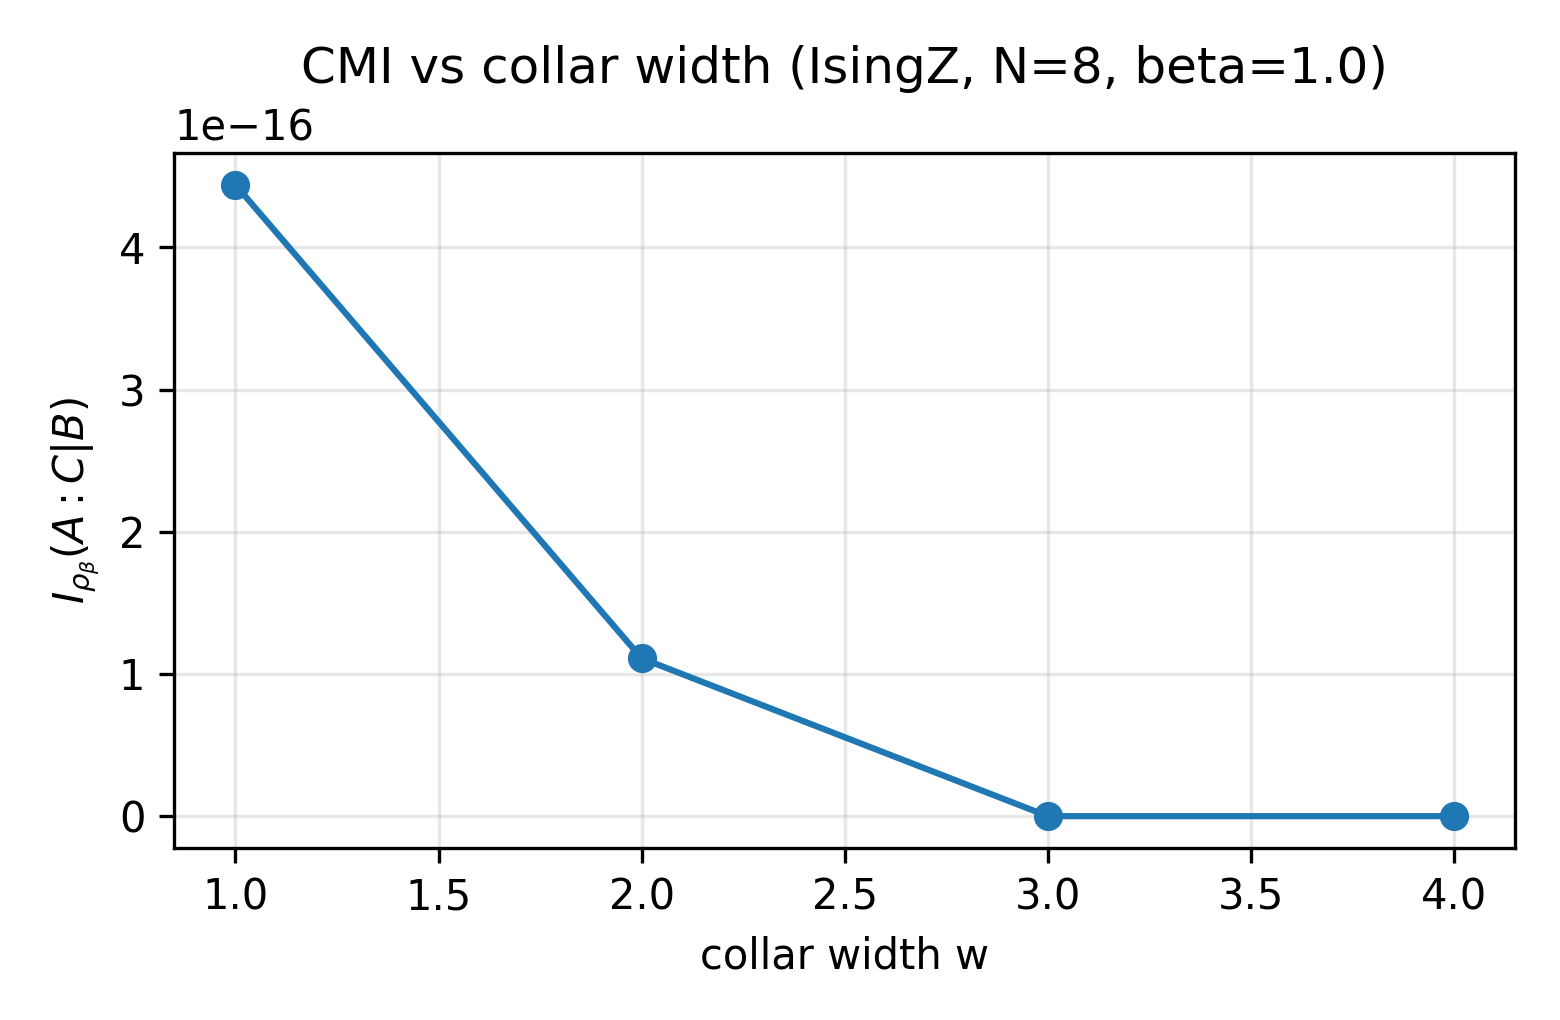
\includegraphics[width=0.72\textwidth]{fig1_cmi_vs_w.png}
\caption{CMI diagnostic: $I_{\rho_\infty}(A:C|B)$ vs collar width $w$
(commuting Ising-Z, $N = 8$, $\beta = 1$). The $10^{-16}$ level reflects
floating-point noise; the suite confirms the exact statement
$I(A:C|B) = 0$ for the 1D Markov field.}
\label{fig:cmi}
\end{figure}
\begin{figure}[h]
\centering
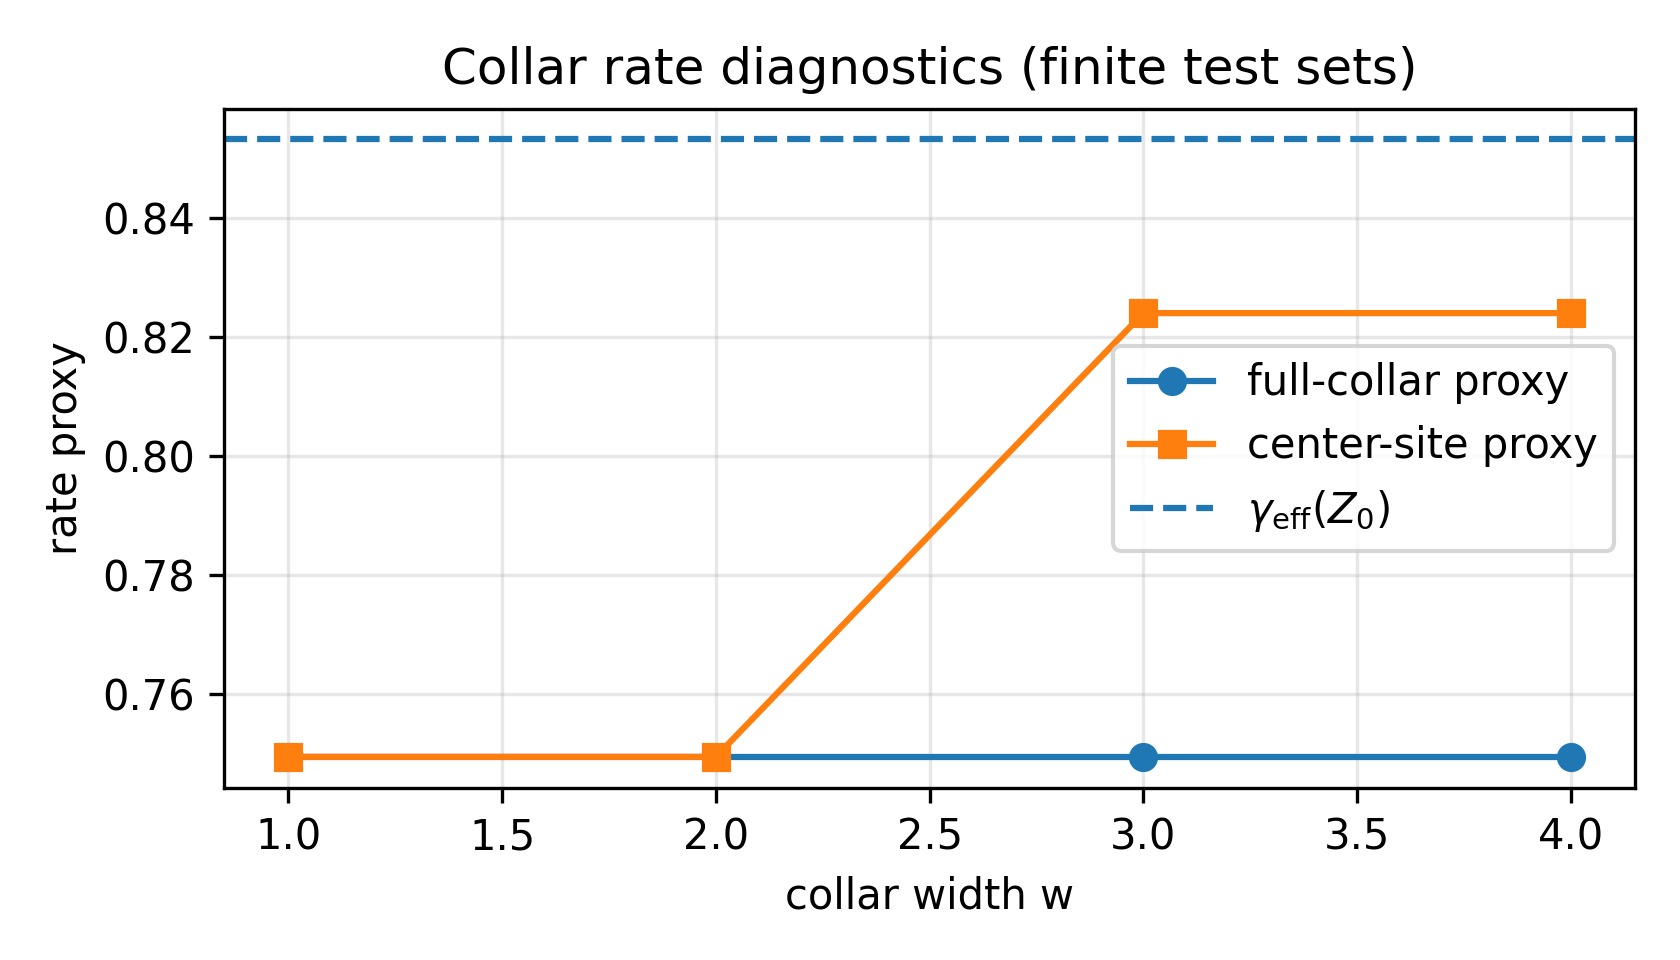
\includegraphics[width=0.8\textwidth]{fig2_collar_diagnostics.png}
\caption{Collar rate diagnostics (finite test sets) for the commuting
Ising-Z heat-bath embedded Lindbladian ($N = 8$, $\beta = 1$).}
\end{figure}

\section{Numerical illustrations (finite-size TFIM)}
These results are illustrative only; no theorem depends on them.
\begin{figure}[h]
\centering
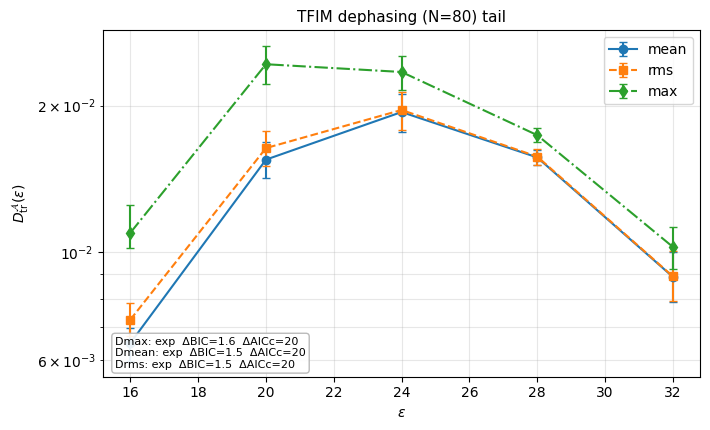
\includegraphics[width=0.6\textwidth]{fig3_tfim_tail.png}
\caption{TFIM dephasing tail ($N = 80$): windowed influence proxy
(illustrative).}
\end{figure}
\begin{figure}[h]
\centering
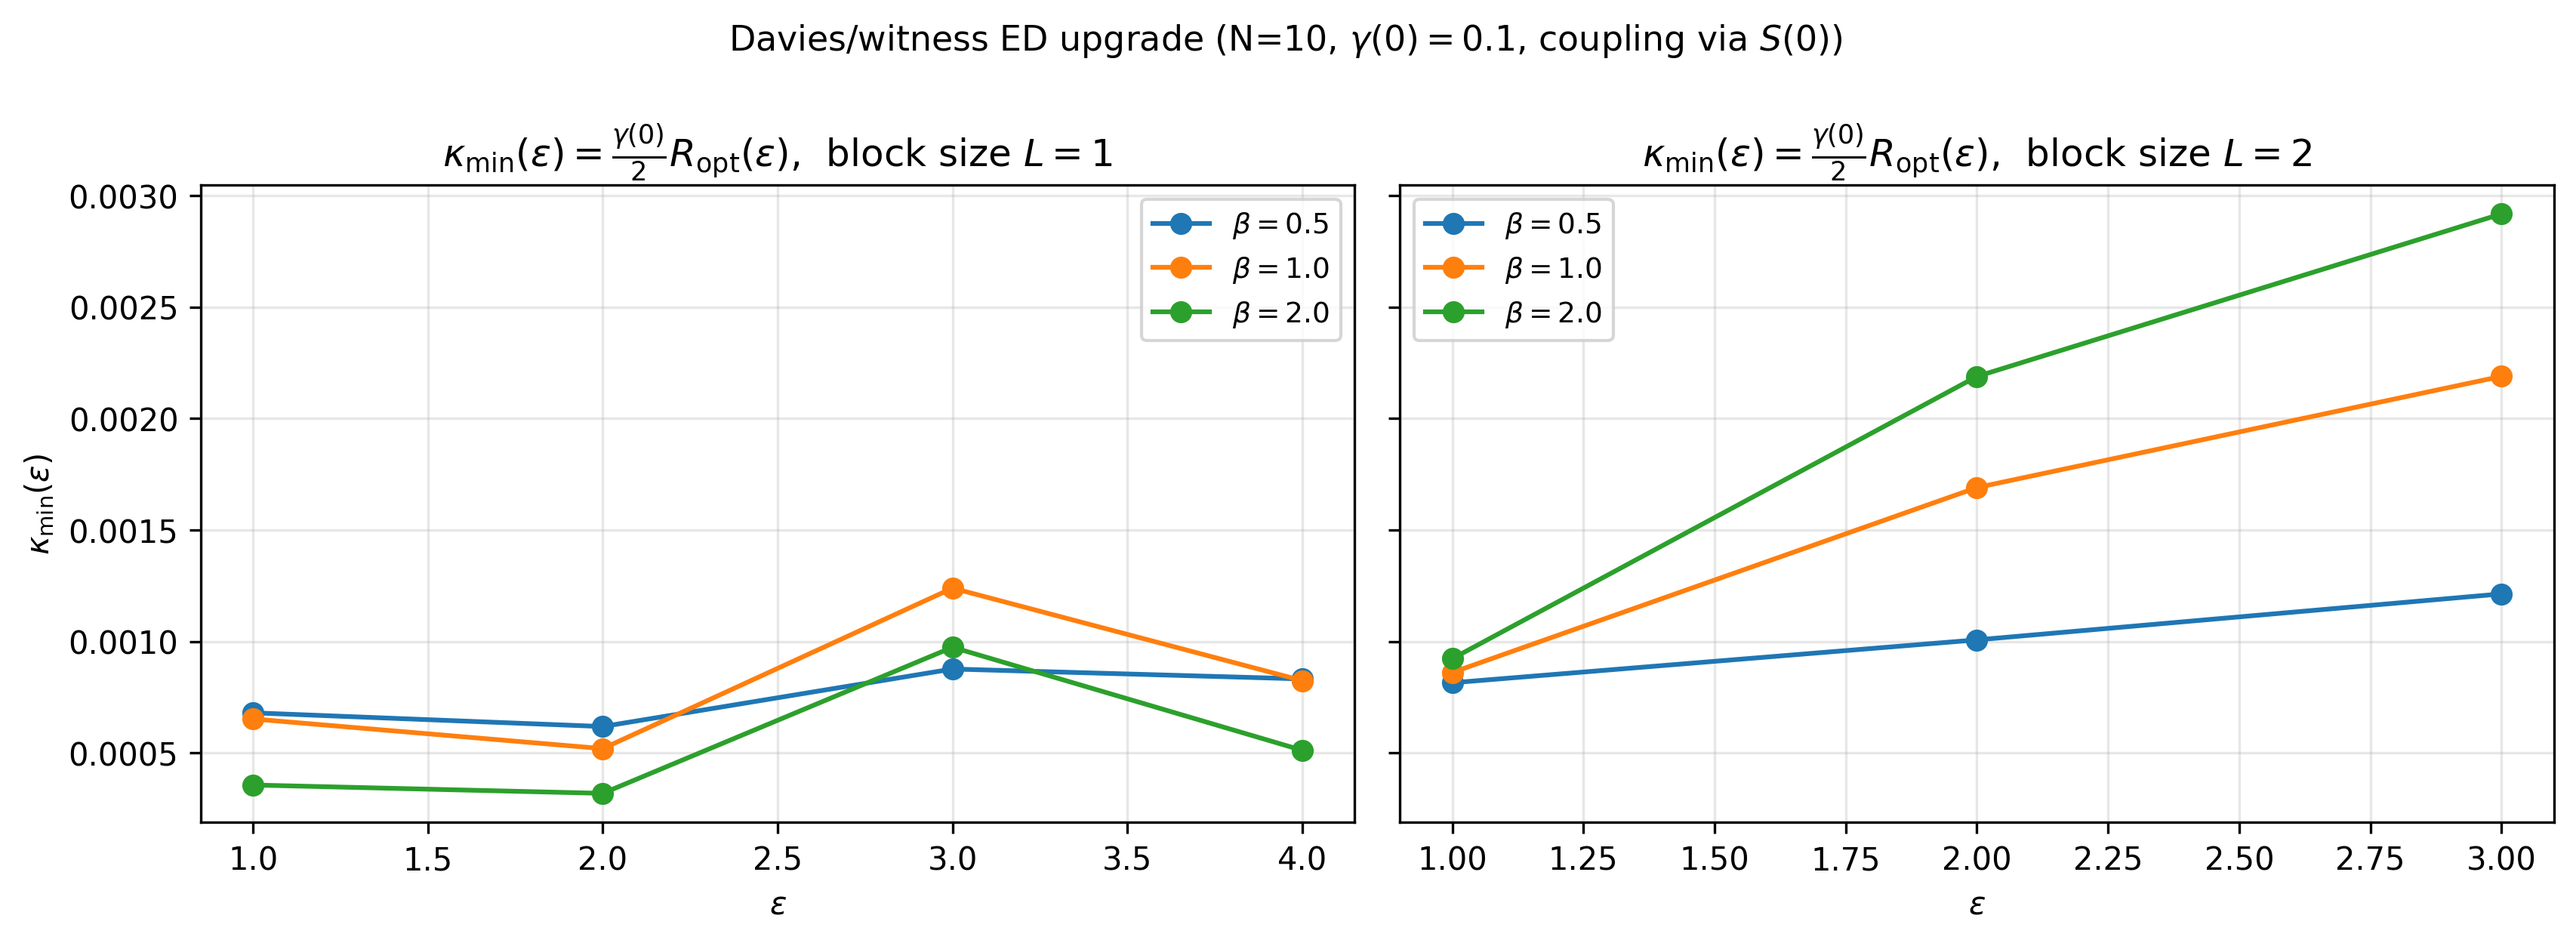
\includegraphics[width=0.8\textwidth]{fig4_witness.png}
\caption{Witness-based lower bound plot (illustrative).}
\end{figure}

\section*{Note added in v2}
Two corrections and one delivery. \emph{Corrections:} (1) the
Fawzi--Renner factor under the squared-fidelity convention is $-\log F$
(Lemma~\ref{lem:fr}, Remark~\ref{rem:frfix}); v1's $-2\log F$ overclaimed,
and Corollary~\ref{cor:georec} now reads $1 - F \le \sigma(\partial B)
g(w)$ (not $\tfrac12\sigma g$). Same correction as 2512.0101 v2. (2) v1's
diagonal bulk--collar comparison (its Proposition A.4) is false as stated
-- exact counterexamples in the suite -- and is replaced by the proved
Proposition~\ref{prop:diagcomp} with extension on $B^{+2r}$
(commuting-projection argument), with Corollary~\ref{cor:diag} restated over the image space $V_A$
(and the 1D boundary-spin degeneracy $\lambda'_B = 0$ for bulk-separated
$A$ identified and flagged); the failure mechanism (range
mismatch at the $B^{+r}$ boundary) is recorded as guidance for
Assumption~\ref{ass:missing}. \emph{Delivery:} the reproducibility item of
v1's own roadmap: full verification suite
(Section~\ref{sec:verif}), series cross-references (Section~2), and the
Figure~1 caption typo fixed.

\begin{thebibliography}{12}
\bibitem{Petz} D. Petz, Commun. Math. Phys. \textbf{105} (1986) 123--131.
\bibitem{FR} O. Fawzi and R. Renner, Commun. Math. Phys. \textbf{340}
(2015) 575--611.
\bibitem{Davies} E. B. Davies, Commun. Math. Phys. \textbf{39} (1974)
91--110.
\bibitem{CR} C.-F. Chen and C. Rouz\'e, \emph{Quantum Gibbs states are
locally Markovian}, arXiv:2504.02208 (2025).
\bibitem{KK} K. Kato and T. Kuwahara, \emph{Clustering of Conditional
Mutual Information via Quantum Belief-Propagation Channels},
arXiv:2504.02235 (2025).
\bibitem{ZG} Y. Zhang and S. Gopalakrishnan, \emph{Conditional Mutual
Information and Information-Theoretic Phases of Decohered Gibbs States},
arXiv:2502.13210 (2025).
\bibitem{S0060} L. Eriksson, ai.viXra:2512.0060 (2025; v2 2026).
\bibitem{S0101} L. Eriksson, ai.viXra:2512.0101 (2025; v2 2026).
\bibitem{S0007} L. Eriksson, ai.viXra:2601.0007 (2026; v2 2026).
\bibitem{S0072} L. Eriksson, ai.viXra:2512.0072 (2025; v2 2026).
\bibitem{S0070} L. Eriksson, ai.viXra:2512.0070 (2025; v2 2026).
\bibitem{S0064} L. Eriksson, ai.viXra:2512.0064 (2025; v2 2026).
\end{thebibliography}
\end{document}
